% !TEX root = ../main.tex
\section{Surge probability: calibration}
\label{sec:calibration}

The model's raw $R$ is \textbf{\ifRawUnderConfident under-confident\else over-confident\fi{} in the middle}: in the reliability bins between \gapBinLo{} and \gapBinHi{}, outcomes came true \ifRawUnderConfident more\else less\fi{} often than forecast, by up to \gapRaw{} (Figure~\ref{fig:reliability}). Isotonic regression maps raw $R$ to the observed surge frequency. It is fitted at each origin on earlier forecasts whose four-week outcome was already known (target week no later than the origin), so it never sees the future. It needs \calMinRows{} past outcomes first: the \nUncalOrigins{} origins before \firstCalOrigin{} keep raw $R$ (\nUncalRows{} rows). After recalibration the largest middle-bin gap is \gapCal{}\ifCalGapSmaller, smaller than before\else, no smaller than before\fi.

\begin{figure}[htbp]
\centering
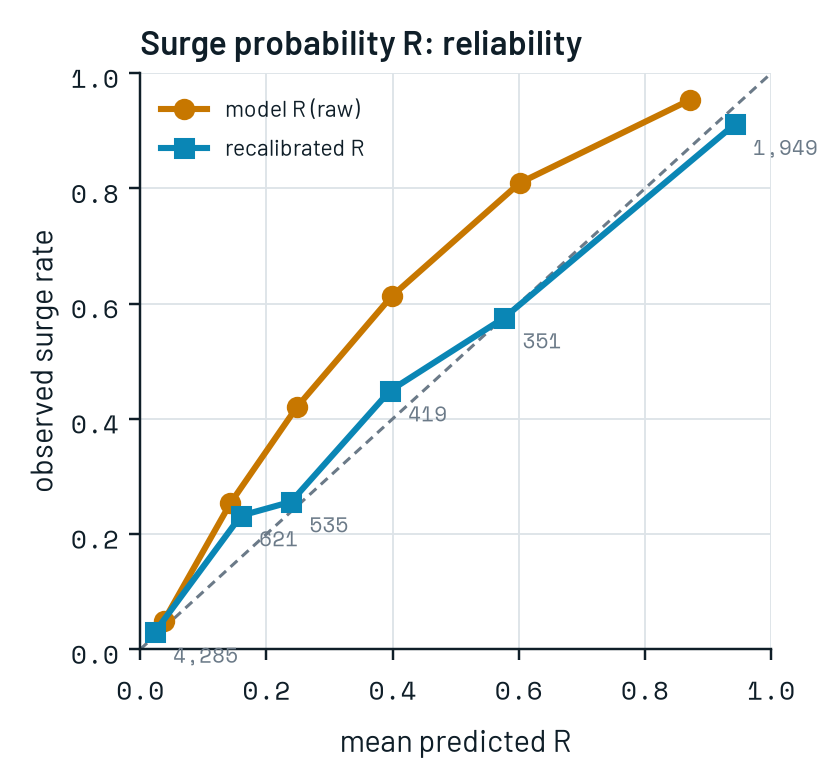
\includegraphics[width=0.5\linewidth]{f04_reliability}
\caption{Reliability of $R$ over the 2018--2019 unit-weeks, before (amber) and after (teal) isotonic recalibration; labels give the unit-weeks per bin.}
\label{fig:reliability}
\end{figure}

Table~\ref{tab:calib} gives the Brier scores: recalibration \ifCalImproves lowers\else raises\fi{} it from \brierRaw{} to \brierCal{} over all 2018--2019 origins. The base rate is \baseRatePct{}\ifBaseRateHigh, not \surgeExpected{}, because 2019 was an epidemic year and the thresholds come from earlier, quieter years\fi. The scenario files keep both \code{R} (calibrated, used for $P$ and the tiers) and \code{R\_raw}. Recalibration changes which provinces reach the provisional tiers (pre-position at $R \geq \tierPreR$, deploy at $R \geq \tierDeployR$ with $A \geq \tierDeployA$): for Ompong the mean $R$ \ifOmpongRRises rises\else falls\fi{} from \ompongRRaw{} to \ompongR{}. The tier thresholds still need review with users.

\begin{table}[htbp]
\centering
\caption{Brier score of $R$ before and after recalibration, against always predicting the base rate.}
\label{tab:calib}
\footnotesize
\begin{tabular}{@{}l r r r r r r r@{}}
\toprule
rows & $n$ & base rate & mean $R$ raw & mean $R$ cal. & Brier raw & Brier cal. & Brier base rate \\
\midrule
\tablerows{calib}
\bottomrule
\end{tabular}
\end{table}

\textbf{Ties.} Isotonic regression is a step function, so provinces share values: for Ompong the \nUnits{} units take \nDistinctR{} distinct values of $R$ and \nTies{} share the top value (\tieValue{}). A ranking by $R$ alone has ties; $P = R \times A$ breaks them by access, and the backtest's Spearman correlations use average ranks.
